% Options for packages loaded elsewhere
\PassOptionsToPackage{unicode}{hyperref}
\PassOptionsToPackage{hyphens}{url}
%
\documentclass[
  9pt,
  ignorenonframetext,
]{beamer}
\usepackage{pgfpages}
% set the section number 
\setbeamertemplate{section in toc}[sections numbered]
\setbeamertemplate{subsection in toc}[subsections numbered]
\setbeamertemplate{navigation symbols}{}
% set the page
\setbeamertemplate{footline}[page number]
\setbeamertemplate{caption}[numbered]
\setbeamertemplate{caption label separator}{: }
\setbeamercolor{caption name}{fg=normal text.fg}
\beamertemplatenavigationsymbolsempty

%%
%%% Definition of colors
%%% Source: https://latexcolor.com/
\definecolor{blanchedalmond}{rgb}{1.0, 0.92, 0.8}
\definecolor{blond}{rgb}{0.98, 0.94, 0.75}
%%% End of definition of colors
%%

% Prevent slide breaks in the middle of a paragraph
\widowpenalties 1 10000
\raggedbottom
\setbeamertemplate{part page}{
  \centering
  \begin{beamercolorbox}[sep=16pt,center]{part title}
    \usebeamerfont{part title}\insertpart\par
  \end{beamercolorbox}
}
\setbeamertemplate{section page}{
  \centering
  \begin{beamercolorbox}[sep=12pt,center]{part title}
    \usebeamerfont{section title}\insertsection\par
  \end{beamercolorbox}
}
\setbeamertemplate{subsection page}{
  \centering
  \begin{beamercolorbox}[sep=8pt,center]{part title}
    \usebeamerfont{subsection title}\insertsubsection\par
  \end{beamercolorbox}
}
\AtBeginPart{
  \frame{\partpage}
}
\AtBeginSection{
  \ifbibliography
  \else
    \frame{\sectionpage}
  \fi
}
\AtBeginSubsection{
  \frame{\subsectionpage}
}
\usepackage{lmodern}
\usepackage{amssymb,amsmath}
\usepackage{ifxetex,ifluatex}
\ifnum 0\ifxetex 1\fi\ifluatex 1\fi=0 % if pdftex
  \usepackage[T1]{fontenc}
  \usepackage[utf8]{inputenc}
  \usepackage{textcomp} % provide euro and other symbols
\else % if luatex or xetex
  \usepackage{unicode-math}
  \defaultfontfeatures{Scale=MatchLowercase}
  \defaultfontfeatures[\rmfamily]{Ligatures=TeX,Scale=1}
\fi
\usetheme[]{Goettingen}
\usecolortheme{rose}
% Use upquote if available, for straight quotes in verbatim environments
\IfFileExists{upquote.sty}{\usepackage{upquote}}{}
\IfFileExists{microtype.sty}{% use microtype if available
  \usepackage[]{microtype}
  \UseMicrotypeSet[protrusion]{basicmath} % disable protrusion for tt fonts
}{}
\makeatletter
\@ifundefined{KOMAClassName}{% if non-KOMA class
  \IfFileExists{parskip.sty}{%
    \usepackage{parskip}
  }{% else
    \setlength{\parindent}{0pt}
    \setlength{\parskip}{6pt plus 2pt minus 1pt}}
}{% if KOMA class
  \KOMAoptions{parskip=half}}
  
% adjust for sidebar
  \setbeamertemplate{sidebar \beamer@sidebarside}
  {
    \beamer@tempdim=\beamer@sidebarwidth%
    \advance\beamer@tempdim by -6pt%
    \vskip4em%
    \insertverticalnavigation{\beamer@sidebarwidth}%
    \vfill
    \ifx\beamer@sidebarside\beamer@lefttext%
    \else%
      \usebeamercolor{normal text}%
      \llap{\usebeamertemplate***{navigation symbols}\hskip0.1cm}%
      \vskip2pt%
    \fi%
  }%

  \ifx\beamer@sidebarside\beamer@lefttext%
    \defbeamertemplate*{sidebar right}{sidebar theme}
    {%
      \vfill%
      \llap{\usebeamertemplate***{navigation symbols}\hskip0.1cm}%
      \vskip2pt}
  \fi

\setbeamertemplate{section in sidebar}%{sidebar theme}
{%
  \vbox{%
    \vskip1ex%
    \beamer@sidebarformat{3pt}{section in sidebar}{\insertsectionheadnumber
~\insertsectionhead}%
  }%
}
\setbeamertemplate{section in sidebar shaded}%{sidebar theme}
{%
  \vbox{%
    \vskip1ex%
    \beamer@sidebarformat{3pt}{section in sidebar shaded}{\insertsectionheadnumber
~\insertsectionhead}%
  }%
}  

\makeatother
\usepackage{xcolor}
\IfFileExists{xurl.sty}{\usepackage{xurl}}{} % add URL line breaks if available
\IfFileExists{bookmark.sty}{\usepackage{bookmark}}{\usepackage{hyperref}}
\hypersetup{
  pdftitle={L1 Introduction},
  pdfauthor={EJC},
  hidelinks,
  pdfcreator={LaTeX via pandoc}}
\urlstyle{same} % disable monospaced font for URLs
\newif\ifbibliography
\setlength{\emergencystretch}{3em} % prevent overfull lines
\providecommand{\tightlist}{%
  \setlength{\itemsep}{0pt}\setlength{\parskip}{0pt}}
\setcounter{secnumdepth}{5}

%
% When using babel or polyglossia with biblatex, loading csquotes is recommended 
% to ensure that quoted texts are typeset according to the rules of your main language.
%
\usepackage{csquotes}

%
% blockquote
%
\definecolor{blockquote-border}{RGB}{221,221,221}
\definecolor{blockquote-text}{RGB}{89,89,89}
\usepackage{mdframed}
\newmdenv[rightline=false,bottomline=false,topline=false,linewidth=3pt,linecolor=blockquote-border,skipabove=\parskip]{customblockquote}
\renewenvironment{quote}{\begin{customblockquote}\list{}{\rightmargin=0em\leftmargin=0em}%
\item\relax\color{blockquote-text}\ignorespaces}{\unskip\unskip\endlist\end{customblockquote}}

%
% Source Sans Pro as the de­fault font fam­ily
% Source Code Pro for monospace text
%
% 'default' option sets the default 
% font family to Source Sans Pro, not \sfdefault.
%
\usepackage[default]{sourcesanspro}
\usepackage{sourcecodepro}

% XeLaTeX specific adjustments for straight quotes: https://tex.stackexchange.com/a/354887
% This issue is already fixed (see https://github.com/silkeh/latex-sourcecodepro/pull/5) but the 
% fix is still unreleased.
% TODO: Remove this workaround when the new version of sourcecodepro is reelased on CTAN.
\ifxetex
\makeatletter
\defaultfontfeatures[\ttfamily]
  { Numbers   = \sourcecodepro@figurestyle,
    Scale     = \SourceCodePro@scale,
    Extension = .otf }
\setmonofont
  [ UprightFont    = *-\sourcecodepro@regstyle,
    ItalicFont     = *-\sourcecodepro@regstyle It,
    BoldFont       = *-\sourcecodepro@boldstyle,
    BoldItalicFont = *-\sourcecodepro@boldstyle It ]
  {SourceCodePro}
\makeatother
\fi

\AtBeginSubsection{}
\AtBeginSection{}

\title{L1 Introduction}
\subtitle{BIOS6643 Longitudinal Data Analysis}
\author{EJC}
\date{}
\institute{Department of Biostatistics \& Informatics}

\begin{document}
\frame{\titlepage}

\begin{frame}
  \begin{columns}
  \column{10cm}
  \tableofcontents
  \end{columns}
\end{frame}
\hypertarget{introduction}{%
\section{Introduction}\label{introduction}}

\begin{frame}{Introduction}
\vspace{\baselineskip}

\begin{block}{Questions}
\protect\hypertarget{questions}{}
\begin{itemize}
\tightlist
\item
  What makes longitudinal data different, so that we need special
  methods?
\item
  What are clustered data?
\item
  What are benefits of longitudinal models? (Or models for clustered
  data)
\item
  Why are longitudinal methods not used more?
\end{itemize}
\end{block}
\end{frame}

\begin{frame}{Longitudinal designs}
\protect\hypertarget{longitudinal-designs}{}
\begin{itemize}
\tightlist
\item
  Designed experiments and observational studies can be applied to
  cross-sectional or longitudinal settings. Here, they are defined for
  the latter.
\item
  A controlled experiment involves an intervention, while an
  observational study does not.
\item
  In many cases a controlled experiment will have one or more true
  treatment groups, along with a `control' group that either receives
  some type of placebo, or does not receive any treatment.
\item
  \textbf{See the course notes for more detail on designed experiments
  versus observational studies.}
\end{itemize}
\end{frame}

\hypertarget{time-series-and-longitudinal-data}{%
\section{Time series and longitudinal
data}\label{time-series-and-longitudinal-data}}

\begin{frame}{Time series and longitudinal data}
\begin{block}{Time series methods (generally)\ldots{}}
\protect\hypertarget{time-series-methods-generally}{}
\begin{itemize}
\tightlist
\item
  focus on modeling one process over time (i.e., one observation taken
  at each time point, across time).
\item
  focus on predicting values of future occurrences.
\end{itemize}

Examples: stock prices, temperature, birth and mortality rates, health
data for individuals (e.g., blood pressure), just to name a few areas.
\end{block}

\begin{block}{Longitudinal methods (generally)\ldots{}}
\protect\hypertarget{longitudinal-methods-generally}{}
\begin{itemize}
\tightlist
\item
  Involve measurements on multiple subjects.
\item
  Assume that the correlation structure is the same across subjects but
  that responses are independent between subjects.
\end{itemize}

Often fewer time points for longitudinal data than time series data.\\
Although analytic methods for time series and longitudinal data differ,
they do have common elements, and the underlying processes that generate
the data are often similar.
\end{block}
\end{frame}

\hypertarget{time-series-data-types-and-examples}{%
\section{Time series data types and
examples}\label{time-series-data-types-and-examples}}

\begin{frame}{Time series data types and examples}
\begin{block}{Stationary processes}
\protect\hypertarget{stationary-processes}{}
\begin{itemize}
\tightlist
\item
  A stationary process \(\{Y_t\}\) has a constant mean (expected value)
  and finite 2nd moment for all times \(t\), and the correlation between
  \(Y_t\) and \(Y_{t+h}\) does not depend on \(t\), for all \(h\).
\item
  Below, data for stationary processes were simulated for the model,
  \(Y_t = \mu + \epsilon_t\) where \(\mu\) is the mean and
  \(\epsilon_t\) are errors that are identically but not necessarily
  independently distributed.
\end{itemize}
\end{block}

\begin{block}{Example 1: Stationary process (iid error)}
\protect\hypertarget{example-1-stationary-process-iid-error}{}
For the simulated data, \(\mu=0\) and
\(\epsilon_t \sim \mathcal {N} (0,\ 0.46)\) for all \(t\).

\tiny

\begin{center}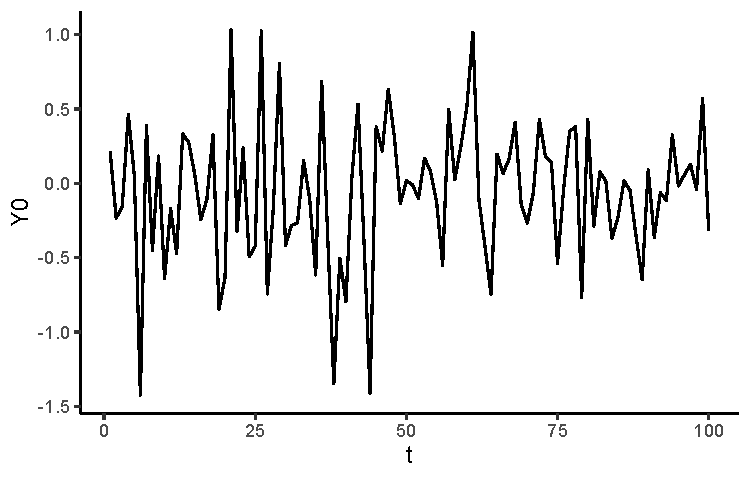
\includegraphics[width=0.5\linewidth]{figs_L1/stationary-1} \end{center}

\tiny
\end{block}
\end{frame}

\begin{frame}{}
\protect\hypertarget{section}{}
\begin{block}{Example 2: Stationary process (correlated error)}
\protect\hypertarget{example-2-stationary-process-correlated-error}{}
\begin{itemize}
\item
  Data below were generated using \(\mu=0\) and errors that followed a
  first-order autoregressive \(\big(AR(1)\big)\) process:
  \(\epsilon_t = \phi\epsilon_{t-1} + Z_t\) and Specifically,
  \(Z_t \stackrel {iid} \sim \mathcal {N} (0,\ 0.46)\), for all \(t\).
\item
  \textbf{Notes on AR(1) processes}:

  \begin{enumerate}
  \tightlist
  \item
    Errors \(\epsilon_t\) are identically distributed but not
    independent
  \item
    Must have \(|\phi| < 1\) for stationary process
  \item
    The higher the value of \(|\phi|\), the higher degree of correlation
    between responses from day to day
  \end{enumerate}
\end{itemize}
\end{block}
\end{frame}

\begin{frame}{}
\protect\hypertarget{section-1}{}
\begin{block}{Example 2: Stationary process (correlated error)}
\protect\hypertarget{example-2-stationary-process-correlated-error-1}{}
\tiny

\begin{center}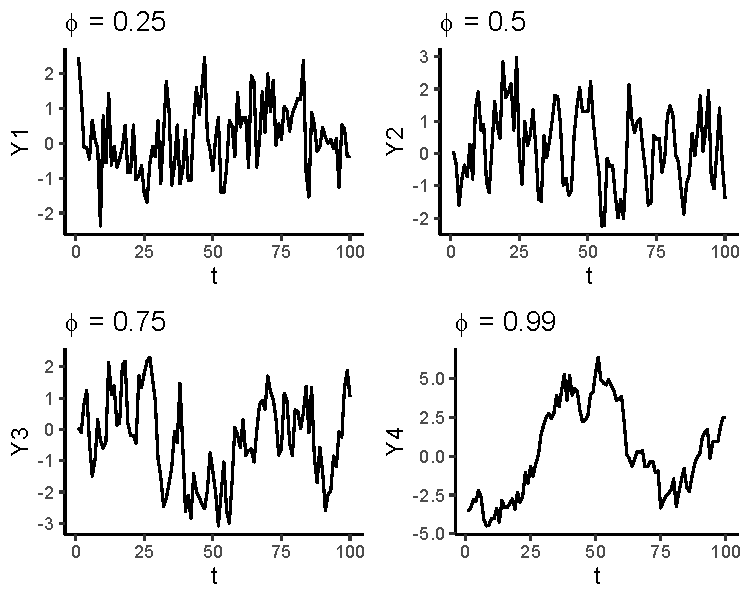
\includegraphics[width=0.9\linewidth]{figs_L1/AR1-1} \end{center}

\tiny
\end{block}
\end{frame}

\begin{frame}{}
\protect\hypertarget{section-2}{}
\begin{block}{Example 3: Processes with trend and correlated errors}
\protect\hypertarget{example-3-processes-with-trend-and-correlated-errors}{}
\begin{itemize}
\tightlist
\item
  \(AR(1)\) process with linear time trend.
\item
  \(Y_t = \beta_0 + \beta_1t + \epsilon_t\), \(\beta_0 = 0\),
  \(\beta_1 = -0.05\), \(\epsilon_t \sim AR(1)\)\\
  (as in \textbf{Example 2}, last page, with \(\phi\ =\ 0.25\))
\end{itemize}

\tiny

\begin{center}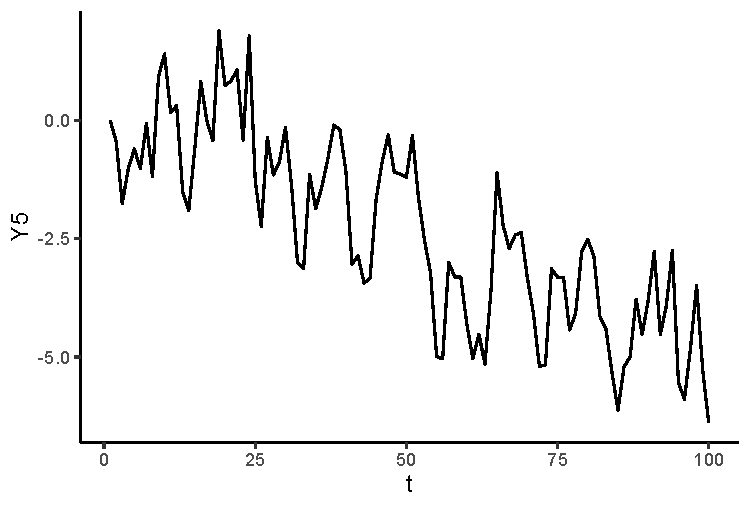
\includegraphics[width=0.5\linewidth]{figs_L1/linear_time_trend-1} \end{center}

\tiny

\textbf{Random walks - see course notes}
\end{block}
\end{frame}

\hypertarget{longitudinal-data-types-and-examples}{%
\section{Longitudinal data types and
examples}\label{longitudinal-data-types-and-examples}}

\begin{frame}{}
\protect\hypertarget{section-3}{}
\begin{block}{Example 4: Observational studies}
\protect\hypertarget{example-4-observational-studies}{}
Longitudinal trajectories of pseudomonas (PA) in EPIC study

\begin{itemize}
\tightlist
\item
  1734 children enrolled in the early pseudomonas infection control
  observational study (EPIC) observational study who were pseudomonas
  negative (PA-)
\item
  Median followup time is 7.8 years (\(Q1 - Q3:\ 6.3 - 8.3\))
\item
  One of the questions of interest was finding factors associated with
  progression of PA; A secondary outcome of interest: time to first
  pulmonary exacerbation in EPIC trial
\end{itemize}

\tiny

\begin{center}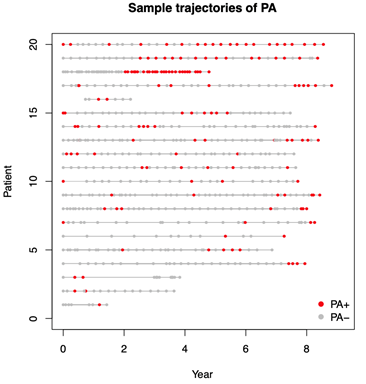
\includegraphics[width=0.5\linewidth]{figs_L1/L1-f1} \end{center}

\tiny
\end{block}
\end{frame}

\begin{frame}{}
\protect\hypertarget{section-4}{}
\begin{block}{Example 5: Prospective randomized trial}
\protect\hypertarget{example-5-prospective-randomized-trial}{}
STEPPED-CARE randomized trial.

\begin{itemize}
\tightlist
\item
  A behavioral intervention was tested versus usual care in 286 patients
  with lung or head and neck cancer.\\
\item
  Population: low income patients in the Denver area across 5 hospitals
\item
  Primary outcomes: anxiety, depression and coping skills scores
\item
  Outcomes were measured at baseline, and at 6, 12 and 24 weeks
\end{itemize}

\vspace{5mm}

\tiny

\begin{center}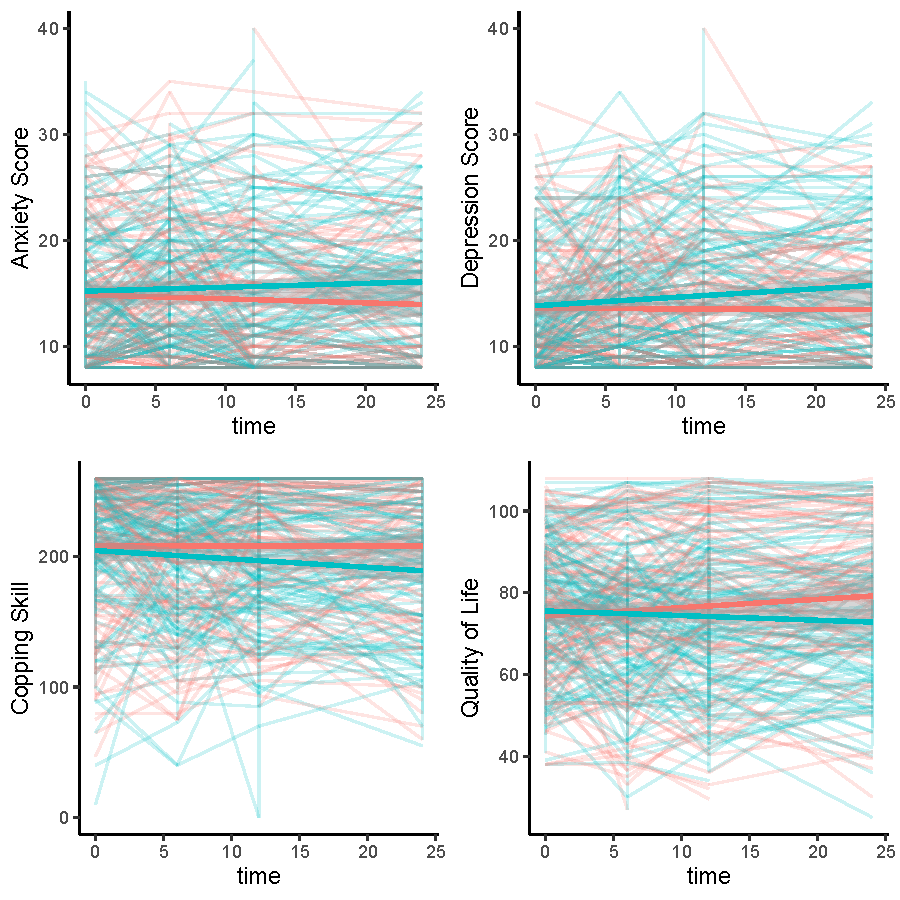
\includegraphics[width=0.5\linewidth]{figs_L1/unnamed-chunk-2-1} \end{center}

\tiny
\end{block}
\end{frame}

\begin{frame}{}
\protect\hypertarget{section-5}{}
\begin{block}{Example 5: Prospective randomized trial}
\protect\hypertarget{example-5-prospective-randomized-trial-1}{}
\tiny

\begin{center}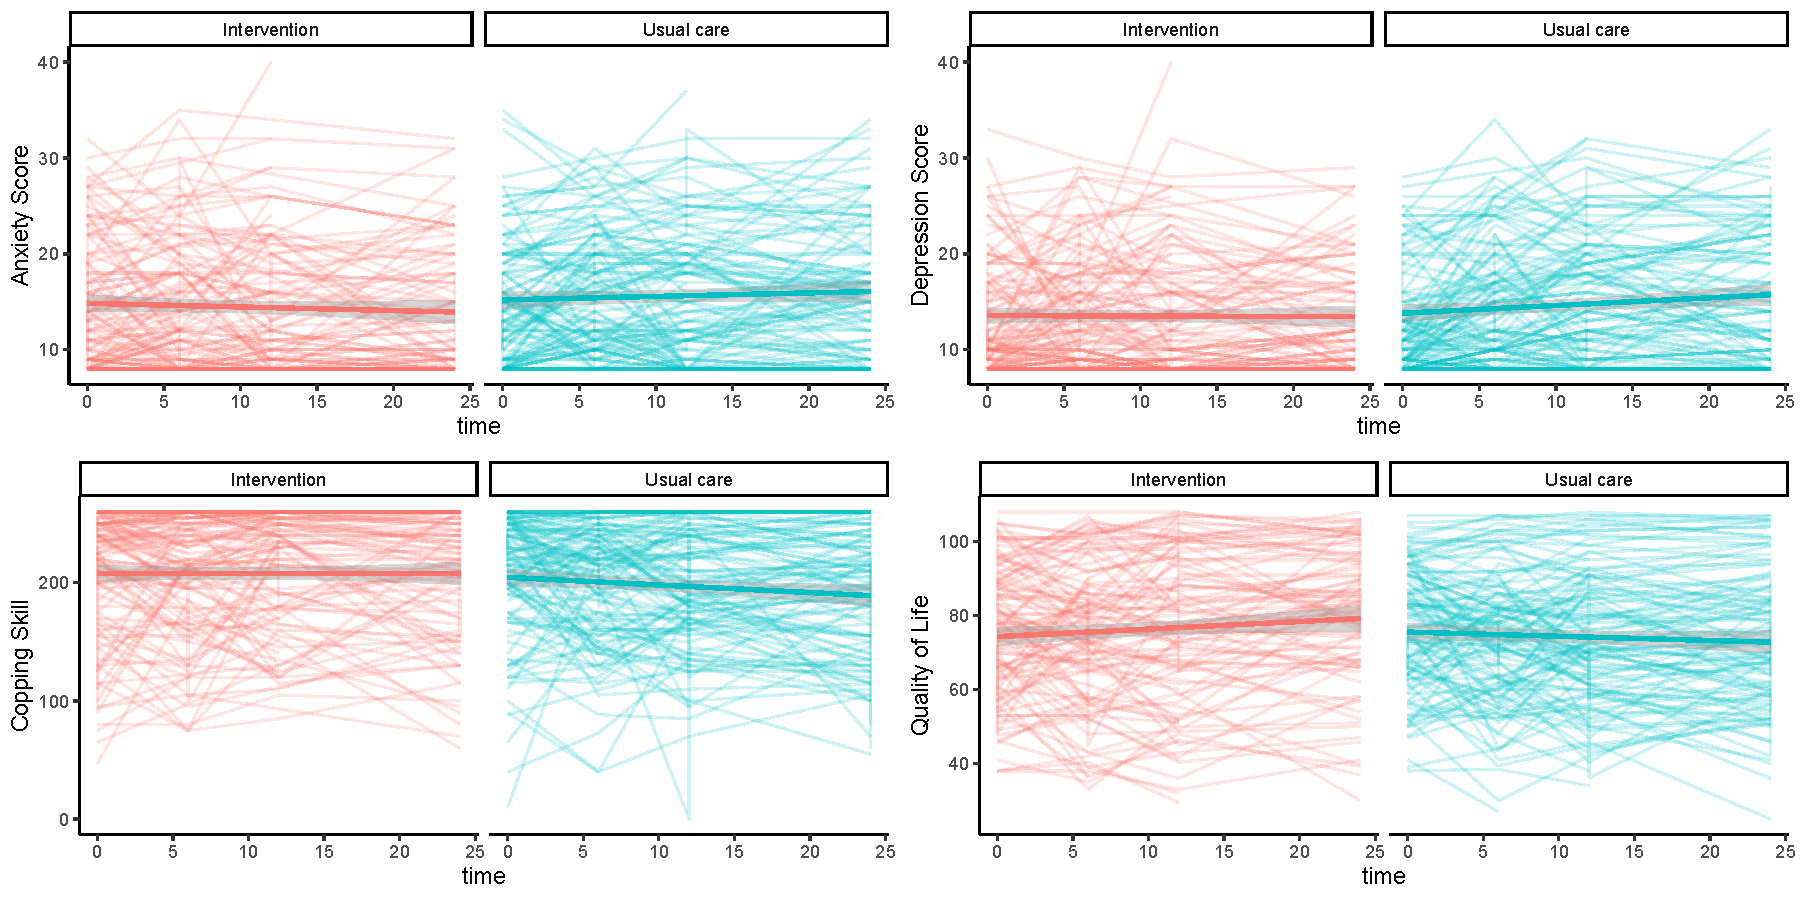
\includegraphics[width=1\linewidth]{figs_L1/unnamed-chunk-3-1} \end{center}

\tiny
\end{block}
\end{frame}

\begin{frame}{}
\protect\hypertarget{section-6}{}
\begin{block}{Example 6: Growth curve data}
\protect\hypertarget{example-6-growth-curve-data}{}
\begin{itemize}
\tightlist
\item
  Graphs for height as a function of age for boys and girls aged 2 to 20
  years
\item
  May be constructed in R using growth data from the
  \href{http://www.cdc.gov/}{CDC}. For more information, please see
  \href{http://www.cdc.gov/growthcharts/}{growcharts}.
\item
  These data show that girls approach their maximum height much more
  quickly than boys. The y-axis scales were made the same for easier
  comparison between graphs.
\item
  Each curve is a percentile estimate as a function of age. We could
  create confidence bands for each percentile curve.\\
\item
  If the curves are estimated using a lot of data, the widths of the
  bands should be narrow. Doctors look for dramatic changes between
  visits.
\item
  The curves here may not be representative of all populations (e.g.,
  differences due to race).
\end{itemize}
\end{block}
\end{frame}

\begin{frame}{}
\protect\hypertarget{section-7}{}
\begin{block}{Example 6: Growth curve data}
\protect\hypertarget{example-6-growth-curve-data-1}{}
\tiny

\begin{center}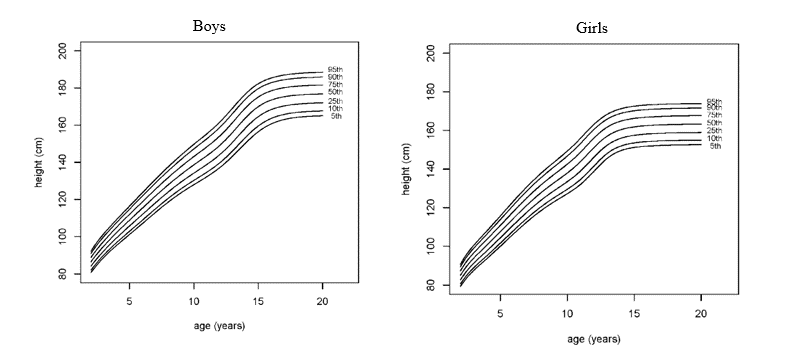
\includegraphics[width=1\linewidth]{figs_L1/L1-f2} \end{center}

\tiny

\textbf{See course notes for more data examples}
\end{block}
\end{frame}

\hypertarget{formats-of-longitudinal-data}{%
\section{Formats of longitudinal
data}\label{formats-of-longitudinal-data}}

\begin{frame}{Formats of longitudinal data}
\begin{itemize}
\tightlist
\item
  ``Univariate'' (long format) versus ``multivariate'' (wide) analysis
\end{itemize}

\tiny

\begin{center}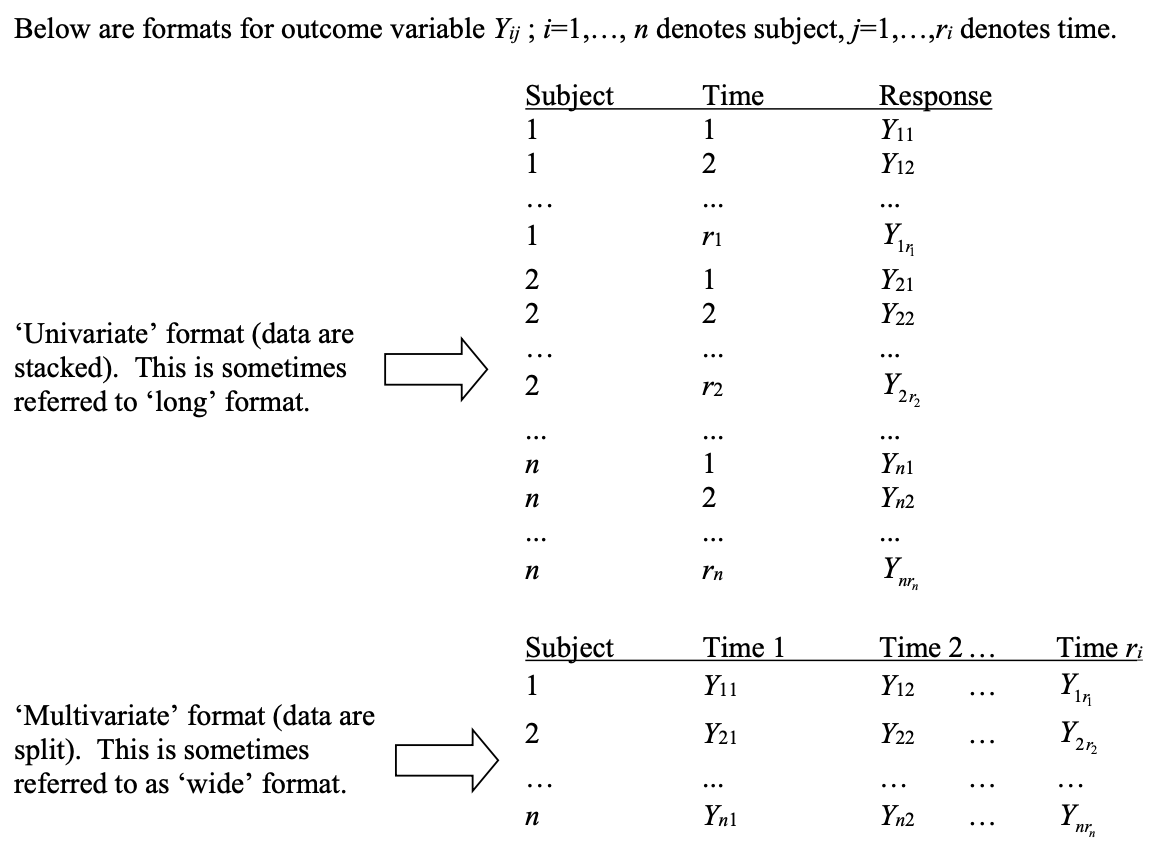
\includegraphics[width=0.6\linewidth]{figs_L1/Fig-L1-formats} \end{center}

\tiny

\begin{itemize}
\tightlist
\item
  See course notes for more information about type of variables and
  notation for variables, e.g.~in longitudinal data versus ``factorial''
  data.
\item
  Factorial data refers to replicated data within each factor and
  treatment combination (think of design of experiments). For example,
  with two factors and replicates within each treatment combinations,
  each replicate needs to be denoted with an index so they outcome could
  be denoted as \(Y_{ijk}\), where \(i\) corresponds to factor, \(j\) to
  the second factor and \(k\) to the replicate
\end{itemize}
\end{frame}

\hypertarget{clusteredlongitudinal-analyses}{%
\section{Clustered/longitudinal
analyses}\label{clusteredlongitudinal-analyses}}

\begin{frame}{Clustered/longitudinal analyses}
\begin{block}{Example 7, 8, \& 9: Cluster data}
\protect\hypertarget{example-7-8-9-cluster-data}{}
\textbf{Example 7}: After an exercise challenge performed on 20
subjects, resting heart rates are monitored at 5 minute intervals for
one hour. How are data clustered?

\textbf{Example 8}: Families are selected to participate in a survey
regarding health insurance.\\
Each member of the family will be included in the study.

\textbf{Example 9}: arm length and leg length growth are measured for
subjects once a year for 10 years, and then modeled with a linear mixed
model.
\end{block}
\end{frame}

\hypertarget{assumptions-of-longitudinal-models}{%
\section{Assumptions of longitudinal
models}\label{assumptions-of-longitudinal-models}}

\begin{frame}{}
\protect\hypertarget{section-8}{}
\begin{itemize}
\item
  Assumption 1: Responses between subjects are independent.

  \begin{itemize}
  \tightlist
  \item
    If there are clear violations to the assumption, and data are
    available, then a random term could be added to deal with this
    non-independence.
  \item
    For example, if there is clustering, e.g.~pairs of siblings in a
    sample, a random term identifying family could be added to the
    model. (Lack of fit and lack of independence are related!)
  \end{itemize}
\item
  Assumption 2: There is a common covariance structure between all
  subjects, and the covariance parameters have the same value between
  subjects.

  \begin{itemize}
  \tightlist
  \item
    This assumption is usually not tested. However, to properly estimate
    covariance parameters, several subjects are needed.
  \item
    In some cases, homogeneous groups within the study may be
    identified. With sufficient group sample sizes, group-specific
    covariance parameters can be put in the model and estimated.
  \end{itemize}
\end{itemize}
\end{frame}

\hypertarget{analyses-of-longitudinal-data-with-two-time-points}{%
\section{Analyses of longitudinal data with two time
points}\label{analyses-of-longitudinal-data-with-two-time-points}}

\begin{frame}{What we've already done!}
\protect\hypertarget{what-weve-already-done}{}
\begin{itemize}
\tightlist
\item
  Experiments with pre-post measurements have 2 measurements on each
  subject over time. When there are only 2 measurements, the analysis
  simplifies when the difference is considered. Simple methods can then
  be used (e.g.~paired t-test).
\item
  Longitudinal models can still be beneficial here! But we'll discuss
  that later. For now, we consider simplified models.
\item
  Let's take a closer look at the underlying models when we use a
  difference score or take the baseline-as-covariate approach.
\end{itemize}

\begin{block}{Change-score model}
\protect\hypertarget{change-score-model}{}
We model the difference using models for univariate outcomes \[
Y_{i1} = Score_{pre}; \ Y_{i2} = Score_{post} 
\] \vspace{-5mm} \[
\Delta_i = Y_{i1} - Y_{i2} = \beta_0 + \beta_1 x_i + \epsilon_i
\]
\end{block}

\begin{block}{Baseline-as-covariate model}
\protect\hypertarget{baseline-as-covariate-model}{}
\[
Y_{i2} = \beta_0 +\beta_1Y_{i1} + \beta_2 x_i + \epsilon_i
\]

We allow the slope of the baseline value to be estimated (based on fit).
\end{block}
\end{frame}

\begin{frame}{}
\protect\hypertarget{section-9}{}
\begin{block}{Example for discussion: cholesterol data}
\protect\hypertarget{example-for-discussion-cholesterol-data}{}
Any other type of simple clustering, with 2 responses per cluster can be
analyzed similarly. (E.g., pairing by married couple, pairing by year of
measurement.)
\end{block}
\end{frame}

\begin{frame}{Longitudinal designs and power - an initial glimpse}
\protect\hypertarget{longitudinal-designs-and-power---an-initial-glimpse}{}
\begin{itemize}
\item
  Consider an experiment designed to compare two treatments. Two common
  approaches:

  \begin{itemize}
  \tightlist
  \item
    A1: Use independent samples (randomly assign some subjects one
    treatment, and some the other). For A1, we often use a 2-independent
    sample t-test
  \item
    A2: Have all subjects take one treatment and then have them all take
    the other (e.g., use a crossover design to eliminate confounding
    effects related to time). For A2, a paired t-test.
  \end{itemize}
\item
  A study/experiment involving changes within subjects (e.g., analyzed
  with a paired t-test) is often more powerful than a study using
  independent samples.
\end{itemize}
\end{frame}

\begin{frame}{}
\protect\hypertarget{section-10}{}
\begin{itemize}
\tightlist
\item
  The general formula for the variance for the difference in means
  suggests why this may be expected (when correlations between responses
  within subjects are positive):
\end{itemize}

\[
Var[\bar Y_1 - \bar Y_2] = Var[\bar Y_1] + Var[\bar Y_2] - 2Cov[\bar Y_1,\ \bar Y_2]
\]

\begin{itemize}
\tightlist
\item
  Often there are many factors not of interest that distinguish the two
  independent samples. For paired data, the difference in responses is
  due more to the treatment alone and not to other factors, since we're
  using the same subjects.\\
\item
  The same principle generalizing to multiple times and longitudinal
  data in general (e.g., air pollution study); subject serve as their
  own controls.
\item
  But paired/longitudinal designs may not always be better. In some
  cases a short cross-sectional study/experiment involving many subjects
  may be more feasible and cost-effective.
\end{itemize}
\end{frame}

\hypertarget{summary}{%
\section{Summary}\label{summary}}

\begin{frame}{Summary}
\protect\hypertarget{summary-1}{}
\begin{itemize}
\tightlist
\item
  Why do we need special methods?
\item
  Discuss time series vs.~longitudinal
\item
  Formats of longitudinal data
\item
  Clustered/longitudinal data
\item
  Assumptions of longitudinal models
\item
  Analyses of longitudinal data with two time points
\end{itemize}
\end{frame}

\end{document}